 
\chapter{An Experimental Perspective of the Instrumental Variable}
 \label{chapter::iv-experiment}



The {\it instrumental variable method} has been a powerful tool in econometrics. It identifies causal effects in studies without unconfoundedness between the treatment and the outcome. It relies on an additional variable, called the {\it instrumental variable} (IV), that satisfies certain conditions. These conditions may not be easy to digest when you learn them for the first time. In some sense, the IV method is like magic. This chapter presents a not-so-magic perspective based on the encouragement design. This again echos \citet{dorn1953philosophy}'s suggestion that the planner of an observational study should always ask himself the following question:\footnote{This quote also appeared in Chapter \ref{chapter::observational-studies} before.}
\begin{quote}
How would the study be conducted if it were possible to do
it by controlled experimentation?
\end{quote} 
The experimental analog of the IV method is {\it noncompliance} in the {\it encouragement design} \citep{zelen1979new, powers1984effects, holland1986statistics}. 



\section{Encouragement Design and Noncompliance}

Consider an experiment with units indexed by $i = 1,\ldots, n$. Let $Z_i$ be the treatment assigned, with $1$ for the treatment and $0$ for the control. Let $D_i$ be the treatment received, with $1$ for the treatment and $0$ for the control.  When $Z_i \neq D_i$ for some unit $i$, the noncompliance problem arises.  Noncompliance is a very common problem, especially in encouragement designs involving human beings as experimental units. In those cases, the experimenters cannot force the units to take the treatment but rather only encourage them to do so. 
Let $Y_i$ be the outcome of interest. 

Consider complete randomization of $Z$ and ignore covariates $X$ for now. We have the potential values for the treatment received $\{  D_i(1), D_i(0) \}$ and  the potential values for the outcome $\{ Y_i(1), Y_i(0)  \}$, all with respect to the treatment assignment levels $1$ and $0$. 
Their observed values are $D_i = Z_i D_i(1) + (1-Z_i) D_i(0)$ and $Y_i = Z_i Y_i(1) + (1-Z_i) Y_i(0)$, respectively. 
For notational simplicity, we assume   $\{  Z_i, D_i(1), D_i(0) ,Y_i(1), Y_i(0)  \}_{i=1}^n \iidsim \{  Z, D(1), D(0) ,Y(1), Y(0)  \}$ and sometimes drop the subscript $i$ when it should not cause confusions. 


We start with the CRE. 
\begin{assumption}[randomization]
\label{assume::random}
$Z\ind \{D(1), D(0) ,Y(1), Y(0)   \}$. 
\end{assumption}

Randomization allows for the identification of the average causal effects on $D$ and $Y$:
$$
\tau_D = E\{  D(1) - D(0) \} = E(D\mid Z=1) - E(D \mid Z=0)
$$
and
$$
\tau_Y = E\{  Y(1) - Y(0) \} = E(Y\mid Z=1) - E(Y\mid Z=0).  
$$
We can use simple difference-in-means estimators $\hat{\tau}_D$ and $\hat{\tau}_Y$ to estimate $\tau_D$ and $\tau_Y$, respectively. 


Reporting the estimate $\hat{\tau}_Y$ with the associated standard error is called the intention-to-treat (ITT) analysis. It estimates the effect of the treatment assignment on the outcome, and the CRE in Assumption \ref{assume::random} justifies this analysis. However, it may not answer the scientific question, that is, the causal effect of the treatment received on the outcome. 




\section{Latent Compliance Status and Effects}

\subsection{Nonparametric identification}


Following \citet{imbens1994identification} and \citet{angrist1996identification}, we stratify the population based on the joint potential values of $U_i = \{  D_i(1), D_i(0) \}$. Because $D$ is binary, we have four possible combinations:
\begin{eqnarray*}
U_i=\left \{ \begin{array} {ll}
\at  , & \text{if} \hspace{2mm} D_i(1)=1 \hspace{2mm} \text{and} \hspace{2mm} D_i(0)=1; \\
\cp  , & \text{if} \hspace{2mm} D_i(1)=1 \hspace{2mm} \text{and} \hspace{2mm} D_i(0)=0; \\
\df  ,& \text{if} \hspace{2mm} D_i(1)=0 \hspace{2mm} \text{and} \hspace{2mm} D_i(0)=1; \\
\nt  , & \text{if} \hspace{2mm} D_i(1)=0 \hspace{2mm} \text{and} \hspace{2mm} D_i(0)=0,
\end{array}
\right.  
\end{eqnarray*}
where ``$\at$'' is for ``always taker,'' ``$\cp$'' is for ``complier,'' ``$\df$'' is for ``defier,'' and ``$\nt$'' is for ``never taker.'' 
Because we cannot observe $D_i(1)$ and $D_i(0)$ simultaneously, $U_i$ is a latent variable for the compliance behavior of unit $i$. 


Based on $U$, we can use the law of total probability to decompose the average causal effect on $Y$ into four terms:
\begin{eqnarray} 
\tau_Y &=& E\{ Y(1) - Y(0) \mid U=\at  \} \pr(U = \at )  \nonumber  \\
&&+ E\{ Y(1) - Y(0) \mid U=\cp   \} \pr(U = \cp ) \nonumber  \\
&&+ E\{ Y(1) - Y(0) \mid U=\df  \} \pr(U = \df ) \nonumber  \\
&&+ E\{ Y(1) - Y(0) \mid U=\nt  \} \pr(U = \nt ) . \label{eq::decompose-ate-y-cace}
\end{eqnarray}  
Therefore, $\tau_Y $ is a weighted average of four latent subgroup effects. We will look into more details of the latent groups below. 



Assumption \ref{assume::Mono} below restricts the third term in \eqref{eq::decompose-ate-y-cace} to be zero. 
\begin{assumption}[monotonicity]
\label{assume::Mono}
$\pr(U_i = \df) = 0$ or $D_i(1)\geq D_i(0)$ for all $i$, that is, there are no defiers. 
\end{assumption}

Assumption \ref{assume::Mono} holds automatically with {\it one-sided noncompliance} when the units assigned to the control arm have no access to the treatment, i.e., $D_i(0) = 0$ for all units. Under randomization, Assumption \ref{assume::Mono} has a testable implication that 
\begin{equation}
\label{eq::test-mono}
\pr(D=1\mid Z=1) \geq \pr(D=1\mid Z=0).
\end{equation}
But Assumption \ref{assume::Mono} is much stronger than the inequality \eqref{eq::test-mono}. The former restricts $D_i(1)$ and $D_i(0)$ at the individual level whereas the latter restricts them only on average. Nevertheless, when the testable implication \eqref{eq::test-mono} holds, we cannot use the observed data to refute Assumption \ref{assume::Mono}. 


Assumption \ref{assume::ER} below restricts the first and last terms in \eqref{eq::decompose-ate-y-cace} to be zero based on the mechanism of the treatment assignment on the outcome through only the treatment received. 
\begin{assumption}[exclusion restriction]
\label{assume::ER}
$Y_i(1) = Y_i(0)$ for always takers with $U_i=\at$ and never takers with $U_i = \nt$. 
\end{assumption}


As equivalent statement of Assumption \ref{assume::ER} is that $D_i(1) =  D_i(0)$ must imply $Y_i(1) =  Y_i(0)$ for all $i$.  It requires that the treatment assignment affects the outcome only if it affects the treatment received. In double-blind RCTs\footnote{In general, it is better to blind the experiment to avoid various biases arising from placebo effects, patients' expectations, etc. In double-blind RCTs, both doctors and patients do not know the treatment; in single-blind RCTs, the patients do not know the treatment but the doctors know. Sometimes, it is impossible to conduct double or even single-blind trials; those trials are called open trials.}, it is biologically plausible because the outcome only depends on the actual treatment received. That is, if the treatment assignment does not change the treatment received, it does not change the outcome either.  It can be violated if the treatment assignment has {\it direct effects}\footnote{I use ``direct effects'' informally here. See more detailed discussion of the concept in Chapters \ref{chapter::mediation} and \ref{chapter::cde} later.} on the outcome, not through the treatment received. For example, some RCTs are not double-blinded, and the treatment assignment can have some unknown pathways to the outcome. 





Under Assumptions  \ref{assume::Mono} and \ref{assume::ER}, the decomposition \eqref{eq::decompose-ate-y-cace} only has the second term :
\begin{eqnarray}
\label{eq::aceY}
\tau_Y  = E\{ Y(1) - Y(0) \mid U=\cp   \} \pr(U = \cp ).
\end{eqnarray}
Similarly, we can decompose the average causal effect on $D$ into four terms:
\begin{eqnarray*}
\tau_D &=& E\{ D(1) - D(0) \mid U=\at  \} \pr(U = \at ) \\
&&+ E\{ D(1) - D(0) \mid U=\cp   \} \pr(U = \cp ) \\
&&+ E\{ D(1) - D(0) \mid U=\df  \} \pr(U = \df ) \\
&&+ E\{ D(1) - D(0) \mid U=\nt  \} \pr(U = \nt )  \\
&=& 0\times \pr(U = \at ) 
+ 1 \times \pr(U = \cp ) 
+ (-1)\times   \pr(U = \df )
+ 0 \times  \pr(U = \nt ) ,
\end{eqnarray*}
which, under Assumption \ref{assume::Mono}, reduces to
\begin{eqnarray}
\label{eq::aceD}
\tau_D  = \pr(U = \cp ) .
\end{eqnarray}
By \eqref{eq::aceD}, the proportion of the compliers $\pi_\cp = \pr(U = \cp)$ equals the average causal effect of the treatment assigned on $D$, an identifiable quantity under the CRE. Although we do not know all the compliers based on the observed data,  we can identify their proportion in the whole population based on \eqref{eq::aceD}. 
Combining \eqref{eq::aceY} and \eqref{eq::aceD}, we have the following result.


\begin{theorem}
\label{thm::CACE-identification}
Under Assumptions \ref{assume::Mono}--\ref{assume::ER}, we have 
$$
E\{ Y(1) - Y(0) \mid U=\cp   \} = \frac{ \tau_Y  }{ \tau_D}
$$
if $\tau_D \neq 0$. 
\end{theorem}


 

Following \citet{imbens1994identification} and \citet{angrist1996identification}, we define a new causal effect below.

\begin{definition}[CACE or LATE]\label{def::CACE}
Define 
$$
\tau_\cp  =  E\{ Y(1) - Y(0) \mid U=\cp   \}  
$$
as the ``complier average causal effect (CACE)'' or the ``local average treatment effect (LATE)''. It has alternative forms:
\begin{eqnarray*}
\tau_\cp  &=&  E\{ Y(1) - Y(0) \mid D(1) = 1 , D(0) = 0  \} \\
&=&    E\{ Y(1) - Y(0) \mid D(1)  >  D(0)    \} . 
\end{eqnarray*}
\end{definition}

The CACE is the average causal effect of $Z$ on $Y$ among compliers with $ D(1) = 1 , D(0) = 0$, or, equivalently, units with $ D(1)  >  D(0)$ under the monotonicity.
Based on Definition \ref{def::CACE}, we can rewrite Theorem \ref{thm::CACE-identification} as
$$
\tau_\cp  = \frac{ \tau_Y  }{ \tau_D} ,
$$
that is, the CACE or LATE equals the ratio of the average causal effects on $Y$ over that on $D$. Under Assumption \ref{assume::random}, we further identify the CACE below.


\begin{corollary}
\label{corollary::identification-CACE}
Under Assumptions \ref{assume::random}--\ref{assume::ER}, we have 
$$
\tau_\cp = \frac{ E(Y\mid Z=1) - E(Y\mid Z=0) }{ E(D\mid Z=1) - E(D \mid Z=0) } .
$$
\end{corollary}


Therefore, under CRE, monotonicity, and exclusion restriction, we can nonparametrically identify the CACE as the ratio of the difference in means of the outcome over the difference in means of the treatment received. 



\subsection{Estimation}
\label{sec::estimation-IV}


Based on Corollary \ref{corollary::identification-CACE},  we can estimate $\tau_\cp$ by a simple ratio 
$$
\hat{\tau}_\cp  = \frac{  \hat{\tau}_Y }{  \hat{\tau}_D  } ,
$$ 
which is called the Wald estimator \citep{wald1940fitting} or the IV estimator. In the above discussion, $Z$ acts as the IV for $D$.   



We can obtain the variance estimator based on the following heuristics (see Example \ref{thm::delta-method}):
$$
\hat{\tau}_\cp - \tau_\cp  = ( \hat{\tau}_Y  -  \tau_\cp\hat{\tau}_D)/\hat{\tau}_D 
\approx  ( \hat{\tau}_Y  -  \tau_\cp\hat{\tau}_D)/ \tau_D 
= \hat{\tau}_A / \tau_D ,
$$ 
where $\hat{\tau}_A$ is the difference-in-means of the adjusted outcome $A_i = Y_i -  \tau_\cp D_i$. So the asymptotic variance of $\hat{\tau}_\cp$ is close to the  variance  of $\hat{\tau}_A$ divided by $\tau_D^2$. 
The variance estimation proceeds in the following steps: 
\begin{enumerate}
%[(\thesection.1)]
\item
obtain the adjusted outcomes $\hat{A}_i =  Y_i -  \hat{\tau}_\cp D_i\ (i=1, \ldots, n)$;

\item
obtain the Neyman-type variance estimate based on the adjusted outcomes:
$$
\hat{V}_{\hat{A}} = \frac{\hat{S}_{\hat{A}}^2(1)}{n_1} + \frac{\hat{S}_{\hat{A}}^2(0)}{n_0},
$$
where $\hat{S}_{\hat{A}}^2(1)$ and $\hat{S}_{\hat{A}}^2(0)$ are the sample variances of the $\hat{A}_i $'s under the treatment and control, respectively; 

\item
obtain the final variance estimator   $ \hat{V}_{\hat{A}} /  \hat{\tau}_D ^2 .$ 
\end{enumerate}


See Problem \ref{problem::var-iv-estimate} for the justification of the above variance estimator. Alternatively, we can also use the bootstrap to approximate the variance of $\hat{\tau}_\cp $.
The following functions can calculate the point estimator $\hat{\tau}_\cp $ and the standard error with the formula $\hat{V}_{\hat{A}} $ and the bootstrap. 

\begin{lstlisting}
## IV point estimator
IV_Wald = function(Z, D, Y)
{
       tau_D = mean(D[Z==1]) - mean(D[Z==0])
       tau_Y = mean(Y[Z==1]) - mean(Y[Z==0])
       CACE  = tau_Y/tau_D
       
       c(tau_D, tau_Y, CACE)
}

## IV se via the delta method
IV_Wald_delta = function(Z, D, Y)
{
       est         = IV_Wald(Z, D, Y)
       AdjustedY   = Y - D*est[3]
       VarAdj      = var(AdjustedY[Z==1])/sum(Z) + 
                          var(AdjustedY[Z==0])/sum(1 - Z)
       
       c(est[3], sqrt(VarAdj)/abs(est[1]))
}

##IV se via the bootstrap
IV_Wald_bootstrap = function(Z, D, Y, n.boot = 200)
{
       est      = IV_Wald(Z, D, Y)
       
       CACEboot  = replicate(n.boot, {
         id.boot = sample(1:length(Z), replace = TRUE)
         IV_Wald(Z[id.boot], D[id.boot], Y[id.boot])[3]
       })
       
       c(est[3], sd(CACEboot))
}
\end{lstlisting}


Under the null hypothesis that $\tau_\cp = 0$, we can approximate the variance by $\hat{V}_Y /  \hat{\tau}_D ^2$, where $\hat{V}_Y$ is the Neyman-type variance estimate for the difference in means of $Y$. This variance estimator is inconsistent if the true $\tau_\cp$ is not zero. Therefore, it works for testing but not for estimation. Nevertheless, it gives insights for the ITT estimator and the Wald estimator. The ITT estimator $\hat{\tau}_Y$ has estimated standard error  $\sqrt{ \hat{V}_Y}$. The Wald estimator $ \hat{\tau}_Y / \hat{\tau}_D$ essentially equals the ITT estimator multiplied by $1/\hat{\tau}_D > 1$, which is larger in magnitude but at the same time, its estimated standard error increases by the same factor. 
Based on the variance estimators $\hat{V}_Y $ and $\hat{V}_Y /  \hat{\tau}_D ^2$, the confidence intervals for $\tau_Y$ and $\tau_\cp$ are
$$
\hat{\tau}_Y \pm z_{1-\alpha/2} \sqrt{ \hat{V}_Y}
$$
and
$$
\hat{\tau}_Y  / \hat{\tau}_D \pm z_{1-\alpha/2} \sqrt{ \hat{V}_Y}  / \hat{\tau}_D
= 
\left( \hat{\tau}_Y \pm z_{1-\alpha/2} \sqrt{ \hat{V}_Y}  \right) / \hat{\tau}_D 
$$
respectively, where $z_{1-\alpha/2}$ is the $1-\alpha/2$ upper quantile of the standard Normal random variable. 
These confidence intervals give the same qualitative conclusions since they will both cover zero or not. In some sense, the IV analysis provides the same qualitative information as the ITT analysis of $Y$ although it involves more complicated procedures.  




\section{Covariates}

\subsection{Covariate adjustment in the CRE}

We now consider completely randomized experiments with covariates and assume 
$$
Z\ind \{ D(1), D(0), Y(1), Y(0), X \}.
$$
With covariates $X$, we can obtain \citet{lin2013}'s estimators $\hat{\tau}_{D,\textsc{L}}$ and $\hat{\tau}_{Y,\textsc{L}}$ for both $D$ and $Y$, resulting in $\hat{\tau}_{\cp, \textsc{L}} = \hat{\tau}_{Y,\textsc{L}} / \hat{\tau}_{D,\textsc{L}}$. 
 We can approximate the asymptotic variance of $\hat{\tau}_{\cp, \textsc{L}} $ using the bootstrap. The following functions can calculate the point estimator $\hat{\tau}_{\cp, \textsc{L}}p $ and the standard error based on the bootstrap. 
 
\begin{lstlisting}
## covariate adjustment in IV analysis
IV_Lin = function(Z, D, Y, X)
{
  X     = scale(as.matrix(X))
  tau_D = lm(D ~ Z + X + Z*X)$coef[2]
  tau_Y = lm(Y ~ Z + X + Z*X)$coef[2]
  CACE  = tau_Y/tau_D
  
  c(tau_D, tau_Y, CACE)
}


##IV_adj se via the bootstrap
IV_Lin_bootstrap = function(Z, D, Y, X, n.boot = 200)
{
  X         = scale(as.matrix(X))
  est       = IV_Lin(Z, D, Y, X)
  CACEboot  = replicate(n.boot, {
    id.boot = sample(1:length(Z), replace = TRUE)
    IV_Lin(Z[id.boot], D[id.boot], Y[id.boot], X[id.boot, ])[3]
  })
  
  c(est[3], sd(CACEboot))
}
\end{lstlisting}

\subsection{Covariates in conditional randomization or unconfounded observational studies}
\label{section::unconfounded-IV}

If randomization holds conditionally, i.e.,
$$
Z\ind \{ D(1), D(0), Y(1), Y(0) \} \mid  X,
$$
then we must adjust for covariates to avoid bias. The analysis is also straightforward since we already have discussed many estimators in Part \ref{part::observational-studies} for estimating the effects of $ Z$ on $D$ and $Y$, respectively. We can just use them in the ratio formula $\hat{\tau}_\cp = \hat{\tau}_Y / \hat{\tau}_D$ and use the bootstrap to approximate the asymptotic variance. 
I do not implement the corresponding estimator and variance estimator but relegate it as Problem \ref{hw::iv-conditional-x}. 



\section{Weak IV}

\subsection{Some simulation}
 
Even if $\tau_D >0$, there is a positive probability that $\hat{\tau}_D$ is zero, so the variance of $\hat{\tau}_\cp$ is infinity (see Problem \ref{problem::infinite-var-iv}). The variance from the Normal approximation discussed before is not the variance of  $\hat{\tau}_\cp$ but rather the variance of its asymptotic distribution. This is a subtle technical point.  When $ \tau_D$ is close to $0$, which is referred to as the weak IV case, the ratio estimator $\hat{\tau}_\cp = \hat{\tau}_Y / \hat{\tau}_D$ has poor finite-sample properties.  In this scenario, $\hat{\tau}_\cp$ has finite-sample bias and non-Normal asymptotic distribution, and the corresponding Wald-type confidence intervals have poor coverage properties\footnote{The theory often assumes that $\tau_D$ has the order $n^{-1/2}$. Under this regime, the proportion of compliers goes to 0 as $n$ goes to infinity. The IV method can only identify a subgroup average causal effect with the proportion shrinking to 0.  This is a contrived regime for theoretical analysis. It is hard to justify this assumption in practice. The following discussion does not assume it.}. In the simple case with a binary outcome $Y$, we know that $\tau_Y$ must be bounded between $-1$ and $1$, but there is no guarantee that $\hat{\tau}_\cp$ is bounded between $-1$ and $1$. 
 

Figures \ref{fig::no-x-iv} and \ref{fig::x-iv} show the histograms of $\hat{\tau}_\cp$ and $\hat{\tau}_{\cp, \textsc{L}}$ over simulation with different $\pi_\cp$. I leave the detailed data-generating processes to the \ri{R} code. From the figures, the distributions of the estimators $\hat{\tau}_\cp$ and $\hat{\tau}_{\cp, \textsc{L}}$ are far from Normal when $\pi_\cp$ equals $0.2$ and $0.1$. Statistical inference based on asymptotic Normality is unlikely to be reliable. 

\begin{figure}
\centering 
\begin{subfigure}[b]{\textwidth}
                \centering
                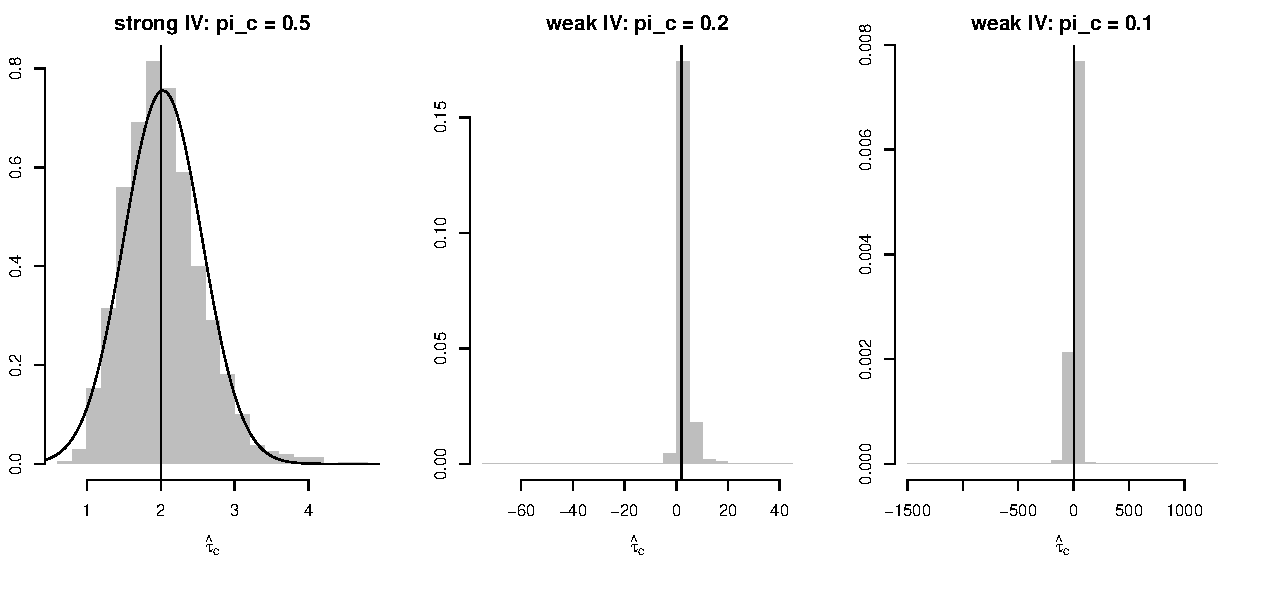
\includegraphics[width=\textwidth]{figures/wald_simulation.pdf}
                \caption{Without covariate adjustment}
                \label{fig::no-x-iv}
        \end{subfigure}%
        
        
        
        
        
        
\begin{subfigure}[b]{\textwidth}
                \centering
                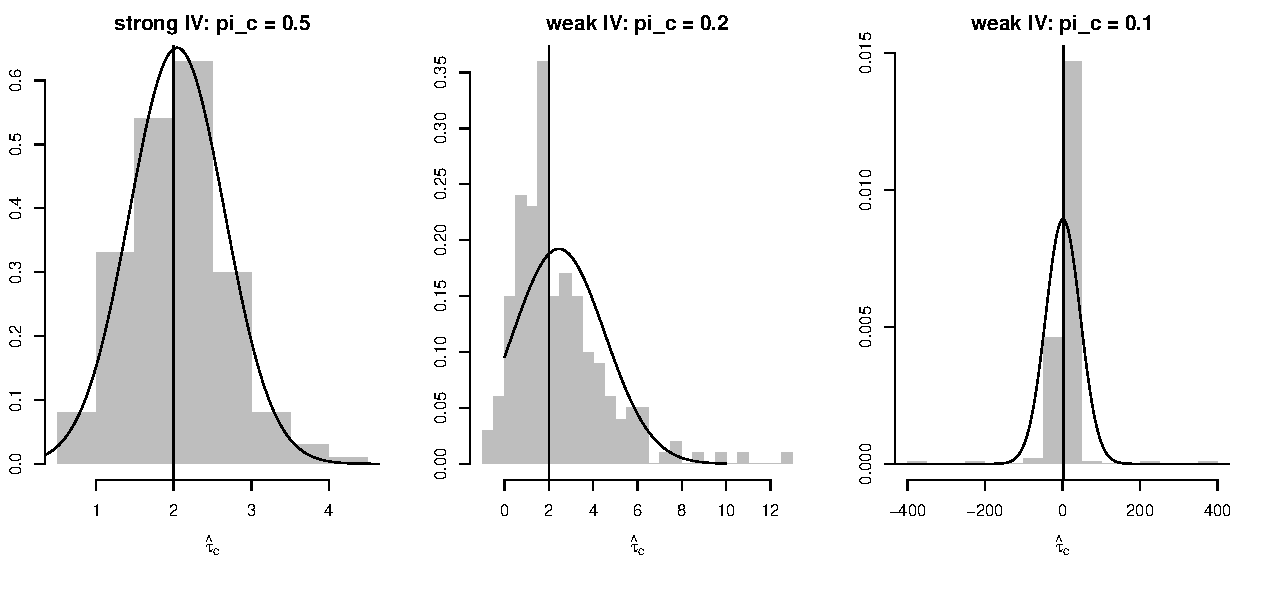
\includegraphics[width=\textwidth]{figures/waldX_simulation.pdf}
                \caption{With covariate adjustment}
                \label{fig::x-iv}
        \end{subfigure}%        
\caption{Simulation with strong and weak IVs}\label{fg::strong-weak-ivs}
\end{figure}


\subsection{A procedure robust to weak IV}

How do we deal with a weak IV?
From a testing perspective, there is an easy solution. Because $\tau_\cp = \tau_Y / \tau_D$, so the following two null hypotheses are equivalent:
$$
H_0: \tau_\cp  = 0 \Longleftrightarrow H_0': \tau_Y = 0
$$
if $\tau_D > 0$. 
Therefore, we simply test $H_0'$, i.e., the average causal effect of $Z$ on $Y$ is zero. This echoes our discussion in Section \ref{sec::estimation-IV} about the relationship between the ITT analysis and the IV analysis. 


From an estimation perspective, we can focus on the confidence interval although the point estimator has poor finite-sample properties. Because $\tau_\cp = \tau_Y / \tau_D$, this is similar to the classical Fieller--Creasy problem in statistics. Below we discuss a strategy for constructing confidence intervals for $\tau_\cp$ motivated by \citet{fieller1954some}; see Chapter \ref{sec::fc-problem}. 
By the duality between confidence intervals and hypothesis tests (See Chapter \ref{section::duality-ci-testing}), we can construct a confidence set for $\tau_\cp$ by inverting a sequence of null hypotheses
$$
H_0(b): \tau_\cp = b . 
$$ 
Given the true value $\tau_\cp = b$, we have
$$
 \tau_Y  - b  \tau_D  = 0.
$$
The null hypothesis $H_0(b)$ is equivalent to the null hypothesis of zero average causal effect on the outcome $A_i( b) = Y_i - b  D_i $:
$$
H_0(b): \tau_{A(b)} = 0 .
$$


Let $ \hat{\tau}_A(b)$ be a generic point estimator for $\tau_{A(b)} $ with the associated variance estimator $\hat{V}_A( b )$. The point and variance estimators depend on the settings. 
In the CRE without covariates, $ \hat{\tau}_A(b)$ is the difference in means of the outcome $A_i( b)$ and $\hat{V}_A( b )$ is the Neyman-type variance estimator. 
In the CRE with covariates, $ \hat{\tau}_A(b)$ is \citet{lin2013}'s estimator for the outcome $A_i( b)$ and $\hat{V}_A( b )$ is the EHW variance estimator in the associated OLS fit of $Y_i - b D_i$ on $(Z_i, X_i, Z_i X_i)$ with the correction term\footnote{If we adopt the finite-population perspective, then we do not need this correction.} discussed in Chapter \ref{sec::cre-superpop}. 
In unconfounded observational studies,  we can obtain the estimator for the average causal effect on $A_i( b)$ and the associated variance estimator based on many existing strategies in Part \ref{part::observational-studies} of the book.  


Based on $ \hat{\tau}_A(b)$ and $\hat{V}_A( b )$, we can construct a Wald-type test for $H_0(b)$. Inverting tests, we can construct the following confidence set for $\tau_\cp$:
$$
\left\{  b:    \frac{   \hat{\tau}_A^2(b)  }{  \hat{V}_A(b)  } \leq z_{1-\alpha/2}^2 \right\}
$$
where $z_{1-\alpha/2}$ is the $1-\alpha/2$ upper quantile of the standard Normal random variable. 
This is close to the Anderson--Rubin-type confidence interval in econometrics \citep{anderson1950asymptotic}.  Due to its connection to \citet{fieller1954some}, I will call it the Fieller--Anderson--Rubin (FAR) confidence interval. 
These weak-IV confidence intervals reduce to the asymptotic confidence intervals when the IV is strong. But they have additional guarantees when the IV is weak. I recommend using them in practice. 


\begin{example}\label{eg::FAR-CI-noX}
To gain intuition about the FAR confidence interval, we look into the simple case of the CRE without covariates. The quadratic inequality in the confidence interval reduces to 
\begin{eqnarray*}
&& (\hat{\tau}_Y  - b   \hat{\tau}_D)^2 \\ 
& \leq & z_{1-\alpha/2}
\left[      n_1^{-1} \{  \hat{S}_Y^2(1)  + b^2\hat{S}_D^2(1) - 2 b \hat{S}_{YD}(1)  \}  \right. \\
&& \left. 
 + n_0^{-1} \{  \hat{S}_Y^2(0)  + b^2\hat{S}_D^2(0) - 2 b \hat{S}_{YD}(0)  \}    \right] ,
\end{eqnarray*}
where $\{ \hat{S}_Y^2(1) ,  \hat{S}_D^2(1) , \hat{S}_{YD}(1)  \}$ and $ \{ \hat{S}_Y^2(0), \hat{S}_D^2(0),\hat{S}_{YD}(0) \} $ are the sample variances and covariances of $Y$ and $D$ under the treatment and control, respectively. 
The confidence set can be a close interval, two disconnected intervals, an empty set, or the whole real line. I relegate the detailed discussion to Problem \ref{para::FAR-CI-cases}. 
\end{example}
 



\subsection{Implementation and simulation}\label{sec::FARci-simulation}


The following functions can compute a sequence of $p$-values as a function of $b$. The function \ri{FARci} does not use covariates, and the function \ri{FARciX} uses covariates which relies on the function \ri{linestimator} defined in Chapter \ref{sec::simulation-CRE-superp}. 

\begin{lstlisting}
FARci = function(Z, D, Y, Lower, Upper, grid)
{
  CIrange = seq(Lower, Upper, grid)
  Pvalue  = sapply(CIrange, function(t){
    Y_t       = Y - t*D
    Tauadj    = mean(Y_t[Z==1]) - mean(Y_t[Z==0])
    VarAdj    = var(Y_t[Z==1])/sum(Z) + 
      var(Y_t[Z==0])/sum(1 - Z)
    Tstat     = Tauadj/sqrt(VarAdj)
    (1 - pnorm(abs(Tstat)))*2
  })
  
  return(list(CIrange = CIrange, Pvalue  = Pvalue))
}

FARciX = function(Z, D, Y, X, Lower, Upper, grid)
{
  CIrange = seq(Lower, Upper, grid)
  X       = scale(X)
  Pvalue  = sapply(CIrange, function(t){
    Y_t       = Y - t*D
    linest    = linestimator(Z, Y_t, X)
    Tstat     = linest[1]/linest[3]
    (1 - pnorm(abs(Tstat)))*2
  })
  
  return(list(CIrange = CIrange, Pvalue  = Pvalue))
}
\end{lstlisting}


Figure \ref{fg::FAR-ci-simulation} displays the $p$-value as a function of $b$ in simulated data with different $\pi_\cp$. Figures \ref{fig::FARci-realization1} and \ref{fig::FARci-realization2} are based on two realizations of the same data-generating process, with details relegated to the \ri{R} code.  In Figure \ref{fig::FARci-realization1}, the FAR confidence sets are all closed intervals, whereas, in Figure \ref{fig::FARci-realization2}, the confidence sets are not closed intervals with $\pi_\cp = 0.2$ and $\pi_\cp = 0.1$. The shapes of the confidence sets remain stable across two realizations with $\pi_\cp = 0.5$. 



\begin{figure}
\centering 
\begin{subfigure}[b]{0.45\textwidth}
                \centering
                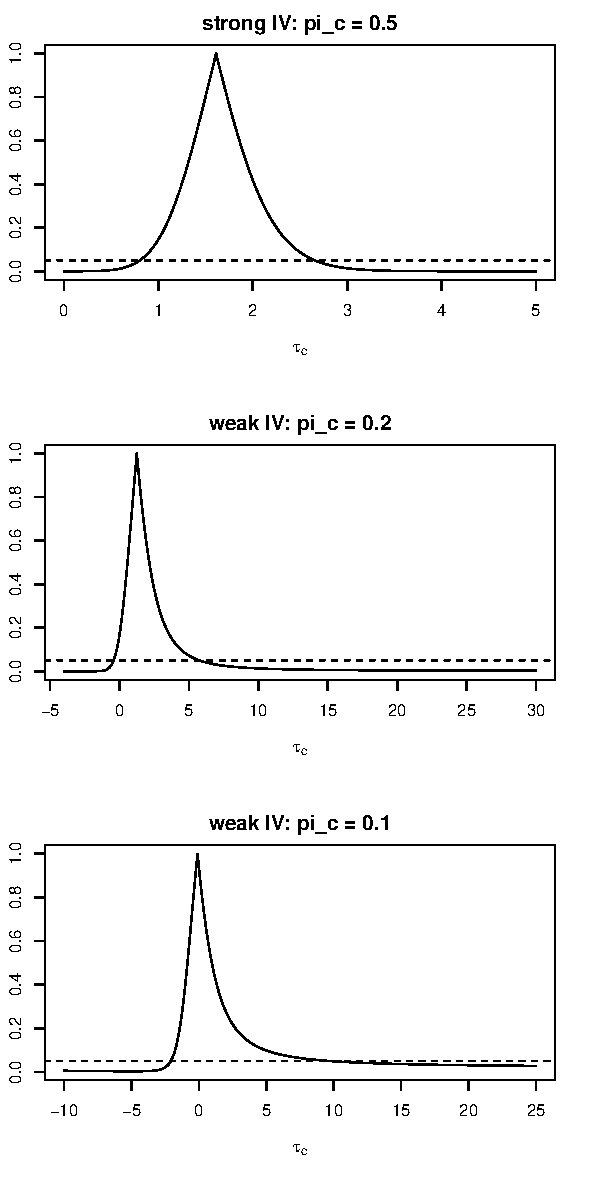
\includegraphics[width=\textwidth]{figures/FARci_simulation1.pdf}
                \caption{Realization 1}
                \label{fig::FARci-realization1}
        \end{subfigure}%
\begin{subfigure}[b]{0.45\textwidth}
                \centering
                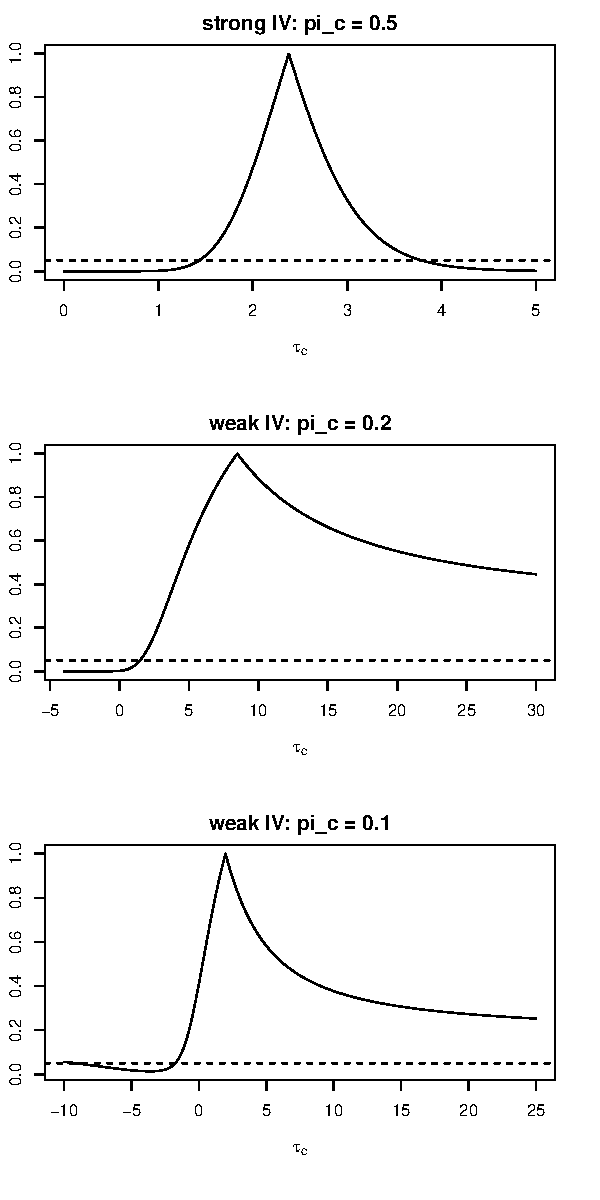
\includegraphics[width=\textwidth]{figures/FARci_simulation2.pdf}
                \caption{Realization 2}
                \label{fig::FARci-realization2}
        \end{subfigure}%        
\caption{FAR confidence interval based on simulated data with different $\pi_\cp$: two realizations}\label{fg::FAR-ci-simulation}
\end{figure}







\section{Application}
\label{sec::cace-application}


The \ri{mediation} package contains a dataset \ri{jobs} from the Job Search Intervention Study (JOBS II), which was a randomized field experiment that investigated the efficacy of a job training intervention on unemployed workers. The variable \ri{treat} is the indicator for whether a participant was randomly selected for the JOBS II training program, and the variable \ri{comply} is the indicator for whether a participant actually participated in the JOBS II program. An outcome of interest is \ri{job_seek} for measuring the level of job-search self-efficacy with values from 1 to 5. Covariates include \ri{sex}, \ri{age}, \ri{marital}, \ri{nonwhite}, \ri{educ}, and \ri{income}. 

 \begin{lstlisting}
> jobsdata = read.csv("jobsdata.csv")
> Z = jobsdata$treat
> D = jobsdata$comply
> Y = jobsdata$job_seek
> getX     = lm(treat ~ sex + age + marital 
+               + nonwhite + educ + income,
+               data = jobsdata)
> X = model.matrix(getX)[, -1]
\end{lstlisting}


We can estimate $\tau_\cp$ by $\hat{\tau}_\cp$ and obtain the standard error based on $\hat{V}_{\hat{A}}$ and the bootstrap. We can further conduct covariate adjustment to obtain $\hat{\tau}_{\cp,\textsc{L}}$ and obtain the standard error based on the bootstrap. The results are below. The point estimator and the standard error are stable across methods. 
 \begin{lstlisting}
> ## without covariates
> res = rbind(IV_Wald_delta(Z, D, Y),
+             IV_Wald_bootstrap(Z, D, Y, n.boot = 10^3))
> ## with covariates 
> res = rbind(res, 
+             IV_Lin_bootstrap(Z, D, Y, X, n.boot = 10^3)) 
> res = cbind(res, res[, 1] - 1.96*res[, 2],
+             res[, 1] + 1.96*res[, 2])
> row.names(res) = c("delta", "bootstrap", "with covariates")
> colnames(res)  = c("est", "se", "lower CI", "upper CI")
> round(res, 3)
                  est    se lower CI upper CI
delta           0.109 0.081   -0.050    0.268
bootstrap       0.109 0.083   -0.054    0.271
with covariates 0.118 0.082   -0.042    0.278
\end{lstlisting}



We can also construct the FAR confidence sets by inverting tests.  They are similar to the confidence intervals above. 
 \begin{lstlisting}
                   lower CI upper CI
without covariates   -0.050    0.267
with covariates      -0.047    0.282
\end{lstlisting}

Figure \ref{fig::FAR-p-value} plots the $p$-values for a sequence of tests. 

\begin{figure}[ht]
\centering
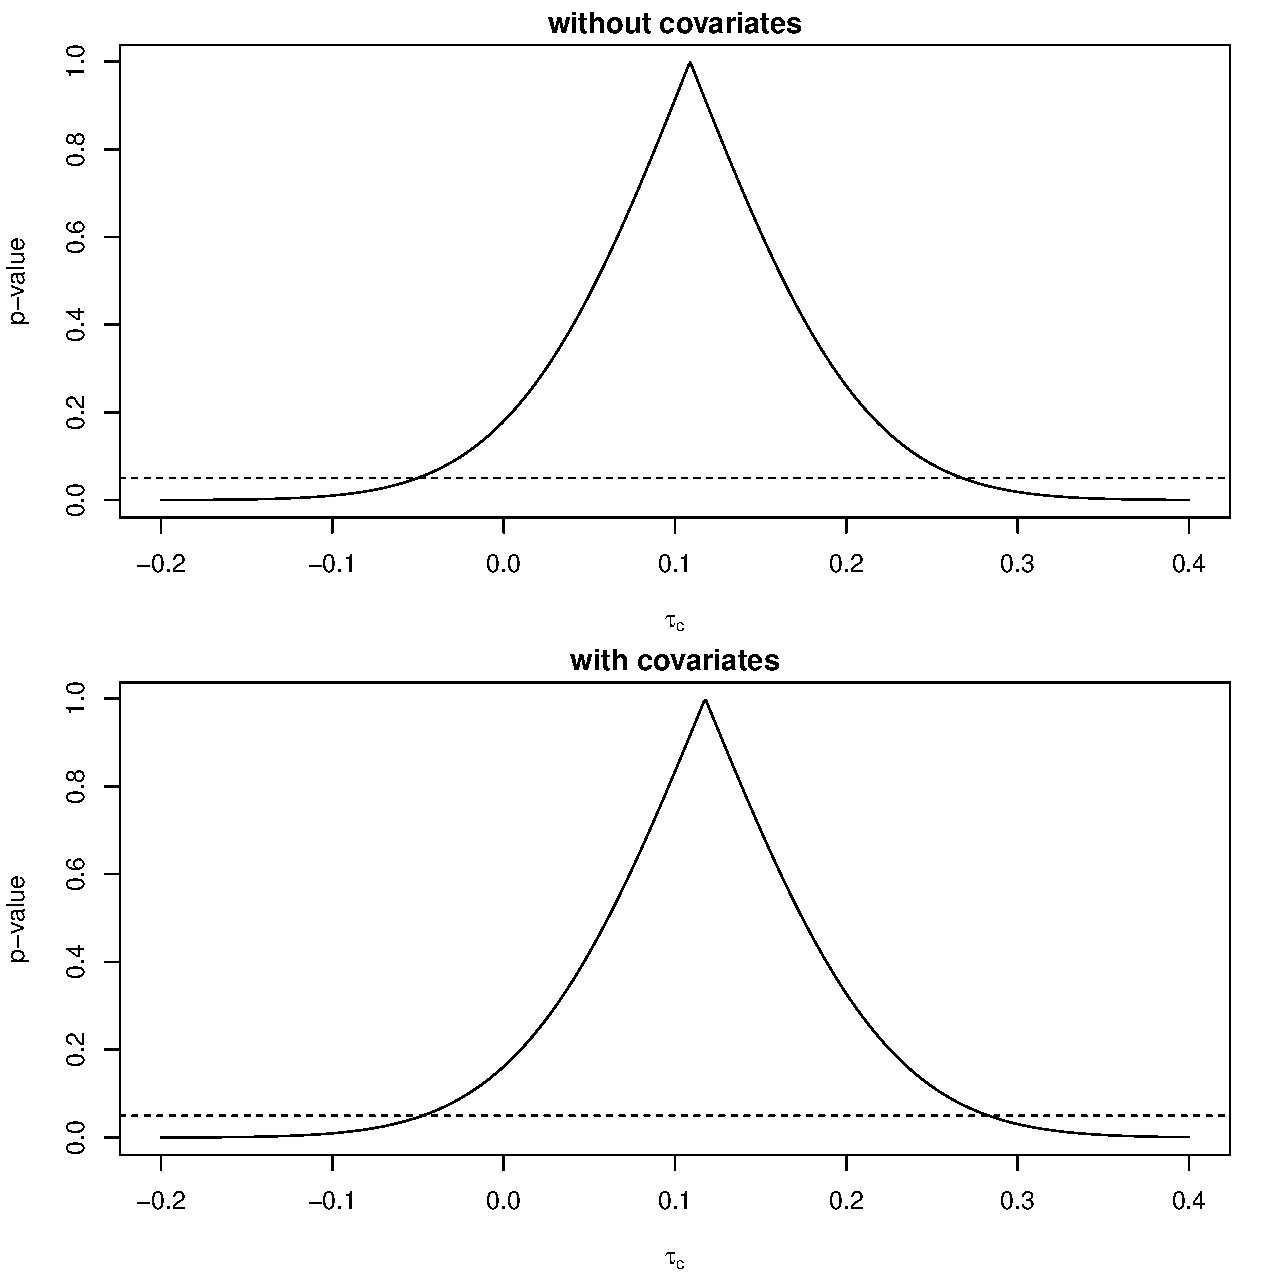
\includegraphics[width = \textwidth]{figures/farci_jobs.pdf}
\caption{Confidence interval of $\tau_\cp$ by inverting tests: upper panel without covariate adjustment, and lower panel with covariate adjustment}\label{fig::FAR-p-value}
\end{figure}




\section{Interpreting the CACE}\label{eq::interpret-iv-double}

The notation for potential outcomes $\{ D(1), D(0), Y(1), Y(0)  \}$ is with respect to the hypothetical intervention of the treatment assigned $Z$. So $\tau_\cp$ is the average causal effect of the treatment assigned on the outcome for compliers. Fortunately, $D=Z$ for compliers, so we can also interpret $\tau_\cp$ as the average causal effect of the treatment received on the outcome for compliers. This partially answers the scientific question. 

 

Some papers use different notation. For instance, \citet{angrist1996identification} use $Y_i(z,d)$ for the potential outcome of unit $i$ under a two-by-two factorial experiment\footnote{The name ``factorial experiment'' is from the experimental design literature \citep{dasgupta2014causal}. The experimenter randomizes multiple factors to each unit. The treatment in the factorial experiment has multiple levels.
} with the treatment assigned $z$ and treatment received $d$. \citet[][Section 3.1]{angrist2022empirical} comments on the intellectual history of this choice of notation. With the notation, the exclusion restriction assumption then has the following form.



\begin{assumption}[exclusion restriction]
\label{assume::ER-double-index}
$Y_i(z,d) = Y_i(d)$ for all $i$, that is, the potential outcome is only a function of $d$.
\end{assumption}


Based on the causal diagram below, Assumption \ref{assume::ER-double-index} rules out the direct arrow from $Z$ to $Y$. In such a case, $Z$ is an IV for $D$. 
\begin{center}
$
\xymatrix{
 && & U  \ar[dl] \ar[dr] &\\
Z \ar[rr] &&D \ar[rr]&&Y
}
$
\end{center}
Under Assumption \ref{assume::ER-double-index}, the augmented notation $Y_i(z,d)$ reduces to $Y_i(d)$, which justifies the name of ``exclusion restriction.'' Therefore, $Y_i(1,d) = Y_i(0,d)$ for $d=0,1$, which, coupled with Assumption \ref{assume::Mono}, implies that
\begin{eqnarray*}
Y_i(z=1) - Y_i(z=0) &=& Y_i(1, D_i(1)) - Y_i(0, D_i(0)) \\
&=& \left \{ \begin{array} {ll}
0 , & \text{if} \hspace{2mm}  U_i = \at, \\
0 , & \text{if}  \hspace{2mm}  U_i = \nt,\\
Y_i(d=1) - Y_i(d=0) ,& \text{if} \hspace{2mm} U_i = \cp.
\end{array}
\right.  
\end{eqnarray*}
In the above, I emphasize the potential outcomes are with respect to $z$, $d$, or both, to avoid confusion. 
The previous decomposition of $\tau_Y$ holds and we have the following result from \citet{imbens1994identification} and \citet{angrist1996identification}.

Recall the average causal effect on $D$, $\tau_D = E\{D(1)  - D(0) \},$ define the average causal effect on $Y$ as $\tau_Y = E\{ Y(D(1)) - Y(D(0))  \}$, and define the complier average causal effect as 
$$
\tau_\cp =  E\{  Y(d=1) - Y(d=0) \mid U = \cp \}.
$$

\begin{theorem}\label{thm::iv-double-index}
Under Assumptions \ref{assume::Mono}--\ref{assume::ER-double-index}, we have 
$$
Y(D(1)) - Y(D(0)) = \{  D(1)  - D(0) \} \times \{ Y(d=1) - Y(d=0) \}
$$
and  
$
\tau_\cp   =   \tau_Y /  \tau_D  .
$
\end{theorem}

The proof is almost identical to the proof of Theorem \ref{thm::CACE-identification} with modifications of the notation. I leave it as Problem \ref{para::iv-alternative-form-theorem}. From the notation $Y_i(d)$, it is more convenient to interpret $\tau_\cp$ as the average causal effect of the treatment received on the outcome for compliers. 



 




 
\section{Homework problems}



 
\paragraph{Variance of the Wald estimator}\label{problem::infinite-var-iv}

Show that $\var(\hat{\tau}_\cp) = \infty$. 



\paragraph{Asymptotic variance of the Wald estimator and its estimation}\label{problem::var-iv-estimate}


Consider the large-sample regime with $n\rightarrow \infty$. 
First show that $\sqrt{n}(\hat{\tau}_\cp - \tau_\cp) \rightarrow \textsc{N}(0, V)$ in distribution and find $V$. Then show that $\hat{V}_{\hat{A}} /V \rightarrow 1$ in probability. 

 
 
 
\paragraph{Proof of the main theorem of  \citet{imbens1994identification} and \citet{angrist1996identification}} 
 \label{para::iv-alternative-form-theorem}
 
 Prove Theorem \ref{thm::iv-double-index}. 
 


\paragraph{More on the FAR confidence set}\label{para::FAR-CI-cases}

The confidence set in Example \ref{eg::FAR-CI-noX} can be a close interval, two disconnected intervals, an empty set, or the whole real line. Find the precise condition for each case.
 
 
 \paragraph{More simulation for the FAR confidence set}\label{para::FAR-CI-simulation-X}

Figure \ref{fg::FAR-ci-simulation} shows the FAR confidence sets without using covariates. Conduct parallel simulation for 
 the FAR confidence sets adjusting for covariates in CRE. 
 
 
\paragraph{Binary IV and ordinal treatment received}\label{para::iv-ordinal-treatment}

\citet{angrist1995two} discussed a more general setting with a binary IV $Z$, an ordinal treatment received $D \in \{0,1,\ldots, J\}$, and an outcome $Y$. The ordinal treatment received has potential outcomes $D(1)$ and $D(0)$ with respect to the binary IV, and the outcome has potential outcomes $Y(z,d)$ with respect to both the binary IV and the ordinal treatment received. Extend the discussion in Section \ref{eq::interpret-iv-double} and the corresponding IV assumptions as below.

\begin{assumption}\label{assumption::iv-ordinal-treatment}
We have
(1) randomization that $Z\ind \{   D(z),  Y(z,d)  : z=0,1; d = 0,1,\ldots, J \}$; 
(2) monotonicity that $D(1) \geq D(0)$; and
(3) exclusion restriction that $Y(z,d) = Y(d)$ for all $z=0,1$ and $ d = 0,1,\ldots, J $. 
\end{assumption}

They proved Theorem \ref{thm::iv-ordinal-treatment} below.

\begin{theorem}\label{thm::iv-ordinal-treatment}
Under Assumption \ref{assumption::iv-ordinal-treatment}, we have 
$$
\frac{  E(Y\mid Z=1) - E(Y\mid Z=0) }{ E(D\mid Z=1) - E(D\mid Z=0)  }
= \sum_{j=1}^J  w_j E\{  Y(j) - Y(j-1)  \mid D(1) \geq j > D(0) \}
$$
where
$$
w_j = \frac{   \pr\{  D(1) \geq j > D(0)   \}   }{   \sum_{j'=1}^J  \pr\{  D(1) \geq j' > D(0)   \}   }.
$$
\end{theorem}



Prove Theorem \ref{thm::iv-ordinal-treatment}.

Remark: 
When $J=1$, Theorem \ref{thm::iv-ordinal-treatment} reduces to Theorem \ref{thm::iv-double-index}. With a general $J$, it states that the standard IV formula identifies a weighted average of some latent subgroup effects. The weights are proportional to the probability of the latent groups defined by $  D(1) \geq j > D(0) $, and the latent subgroup effect $E\{  Y(j) - Y(j-1)  \mid D(1) \geq j > D(0) \}$ compares the adjacent levels of the treatment received. However, this weighted average may not be easy to interpret because the latent groups overlap.



The proof can be tedious. 
A trick is to write the treatment received and outcome under treatment assignment $z$ as 
$$
D(z) = \sum_{j=0}^J j 1\{ D(z) = j\} ,\quad 
Y(D(z)) = \sum_{j=0}^J  Y(j)1\{ D(z) = j\} 
$$
to obtain
$$
D(1) - D(0) = \sum_{j=0}^J j [ 1\{ D(1) = j\} -1\{ D(0) = j\} ]
$$
and
$$
 Y(D(1))  - Y(D(0))   = 
\sum_{j=0}^J Y(j)   [ 1\{ D(1) = j \}   - 1\{ D(0) = j \}  ].
$$
Then use the following {\it Abel's lemma}, also called {\it summation by parts}: 
$$
\sum_{j=0}^J  f_j (g_{j+1} - g_j) 
= 
f_J g_{J+1} - f_0 g_0  - \sum_{j=1}^J g_j  (f_j - f_{j-1})
$$
for appropriately specified sequences $(f_j)$ and $(g_j)$. 





 
 


\paragraph{Data analysis: a flu shot encouragement design \citep{mcdonald1992effects}}\label{problem::flushot}
 

The dataset in \ri{fludata.txt} is from a randomized encouragement design of \citet{mcdonald1992effects}, which was also re-analyzed by \citet{hirano2000assessing}. It contains the following variables:

\begin{tabular}{ll}
\hline 
\texttt{assign} & binary encouragement to receive the flu shot\\
\texttt{receive} & binary indicator for receiving the flu shot \\
\texttt{outcome} & binary outcome for flu-related hospitalization\\
\texttt{age} & age of the patient\\
\texttt{sex} & sex of the patient\\
\texttt{race} & race of the patient\\
\texttt{copd} &  chronic obstructive pulmonary disease\\
\texttt{dm} & diabetes\\
\texttt{heartd} & heart  disease\\
\texttt{renal} & renal  disease\\
\texttt{liverd} & liver  disease\\
\hline 
\end{tabular}


Analyze the data with and without adjusting for the covariates. 
 


\paragraph{IV estimation conditional on covariates}\label{hw::iv-conditional-x}

Implement the estimators and corresponding variance estimators mentioned in Chapter \ref{section::unconfounded-IV} in \ri{R}. 

Remark: The problem is useful for Problem \ref{hw::analyze-karolinska-iv}. 



\paragraph{Data analysis: the Karolinska data}\label{hw::analyze-karolinska-iv}

Revisit Problem \ref{hw::Karolinska-dr}. 
\citet{rubin2008objective} used the Karolinska data as an example for the IV method. In \texttt{karolinska.txt}, whether a patient was diagnosed at a large volume hospital can be viewed as an IV for whether a patient was treated at a large volume hospital. This is plausible conditional on other observed covariates. See \citet{rubin2008objective}'s analysis for more details. 


Re-analyze the data assuming that the IV is randomly assigned conditional on observed covariates. 

 
 
 \paragraph{Data analysis: a job training program}

The file \texttt{jobtraining.rtf} contains the description of the data files \texttt{X.csv} and \texttt{Y.csv}. 

The dataset \texttt{X.csv} contains the pretreatment covariates. You can view the sampling weight variable \texttt{wgt} as a covariate too. Many previous analyses made this simplification although this is always a controversial issue in statistical analysis of survey data. 
Conduct analyses with and without covariates. 

The dataset \texttt{Y.csv} contains the sampling weight, treatment assigned, treatment received, and many post-treatment variables. Therefore, this dataset contains many outcomes depending on your questions of interest. The data also have many complications. First, some outcomes are missing. Second, unemployed individuals do not have wages. Third, the outcomes are repeatedly observed over time. When you analyze the data, please give details about your choice of the questions of interest and estimators. 

Remark: 
\citet{schochet2008does} analyzed the original data.
\citet{frumento2012evaluating} provided a more sophisticated analysis based on the framework in Chapter \ref{chapter::principal-stratification} later. 


 \paragraph{Recommended reading}

\citet{angrist1996identification} bridged the econometric IV perspective and statistical causal inference based on potential outcomes and demonstrated its usefulness with an application. 

Some other early references on IV are \citet{permutt1989simultaneous},  \citet{sommer1991estimating}, \citet{baker1994paired}, and \citet{cuzick1997adjusting}. 


